\documentclass[10pt,twocolumn,letterpaper]{article}
%\documentclass[10pt,onecolumn,letterpaper]{article}
%
\usepackage{iccv}
\usepackage{times}
\usepackage{epsfig}
\usepackage{graphicx}
\usepackage{amsmath}
\usepackage{amssymb}
% ==== extra packages
\usepackage{enumitem}
\usepackage{comment}
% Include other packages here, before hyperref.

% If you comment hyperref and then uncomment it, you should delete
% egpaper.aux before re-running latex.  (Or just hit 'q' on the first latex
% run, let it finish, and you should be clear).
\usepackage[pagebackref=true,breaklinks=true,letterpaper=true,colorlinks,bookmarks=false]{hyperref}

% \iccvfinalcopy % *** Uncomment this line for the final submission

\def\iccvPaperID{328} % *** Enter the ICCV Paper ID here
\def\httilde{\mbox{\tt\raisebox{-.5ex}{\symbol{126}}}}

% Pages are numbered in submission mode, and unnumbered in camera-ready
\ificcvfinal\pagestyle{empty}\fi
%
% ==================== I added these new command 
\newcommand{\myred}{\color{red}}
%% after the reviewing is done, replace the above command with the following one:
% \newcommand{\myred}{\color{black}}
%
\newcommand{\myblue}{\color{blue}}
%\newcomand{\myblue}{\color{black}}
%
\begin{document}

%%%%%%%%% TITLE
\title{Action Recognition with Semantic Attention Convolutional Neural Network}
%
\author{Yunfeng Wang\\
University of Science and Technology of China\\
Institution1 address\\
{\tt\small wangyf11@mail.ustc.edu.cn}
% For a paper whose authors are all at the same institution,
% omit the following lines up until the closing ``}''.
% Additional authors and addresses can be added with ``\and'',
% just like the second author.
% To save space, use either the email address or home page, not both
\and
Second Author\\
Institution2\\
First line of institution2 address\\
{\tt\small secondauthor@i2.org}
}

\maketitle
%\thispagestyle{empty}


%%%%%%%%% ABSTRACT
\begin{abstract}
Spatio-temporal cues and contexts are crucial in understanding human actions in videos. In this paper, a new holistic spatio-temporal method is proposed to simultaneously capture multiple spatial and temporal cues (e.g., human poses, occurrences of objects in the background) with a two-stream Convolutional Neural Network (ConvNet) architecture. The proposed ``Semantic Attention'' ConvNet captures action semantics and spatial attention by combining discriminative information from both the primary region (foreground) and secondary regions (mostly background). In addition, the proposed method is compatible with the conventional RGB image inputs, the optical flow image inputs and both combined, making it flexible to input formats. With optical flow inputs augmenting the RGB inputs, our combined framework achieves evident performance advantages on two challenging public datasets \cite{soomro2012ucf101,Kuehne11}. Even without the optional optical flow inputs, the proposed Semantic Attention ConvNet nevertheless outperforms competing ones on the UCF101~\cite{soomro2012ucf101} dataset. 
%
\end{abstract}



%%%%%%%%% BODY TEXT
\section{Introduction}
Human action recognition is a booming area of computer vision research, due to its widespread applications in human-computer interaction, video surveillance, video game control, \etc. Partially due to the large intraclass variations, action recognition with complex backgrounds remains a challenging task. Generally, there are two types of popular action recognition methods, one based on the handcrafted conventional features and the other based on deep learning. Among the former type, the iDT descriptors \cite{wang2013action} with Fisher vector encoding achieves the highest accuracy. However, this approach is computational demanding since it requires the extraction of dense video trajectories. Alternatively, deep learning based multi-modal/multi-task methods have received tremendous attention in recent years. Conventional feature based multi-modal/multi-task visual recognition \cite{zhang2015can,zhang2015auxiliary,zhang2015multi} has been popular since decades ago. Recently, multi-modal deep learning such as ``Two-Stream~\cite{simonyan2014two}'' and its derivatives \cite{Feichtenhofer16, wang2016two,WangQT15a, sun2015human, wang2016temporal} are among the top performers on the UCF101~\cite{soomro2012ucf101} and HMDB51~\cite{Kuehne11} action recognition dataset. 
%


Despite the successes in leading the benchmark scoreboard, these multi-modal deep learning based methods lack a holistic way of incorporating context information in video frames. Traditionally viewed as a source of noise, the background itself arguably offers valuable hints to recognize the characteristics of the human actions. A typical example is illustrated in Figure~\ref{bask_vs} (b). Even with the basketball player completely censored, the indoor scene of the basketball court (especially the mid-air ball) provides substantial clues to recognize the ``playing basketball'' action. 
%
%-------------------------
\begin{figure*}[t]
\begin{center}
%
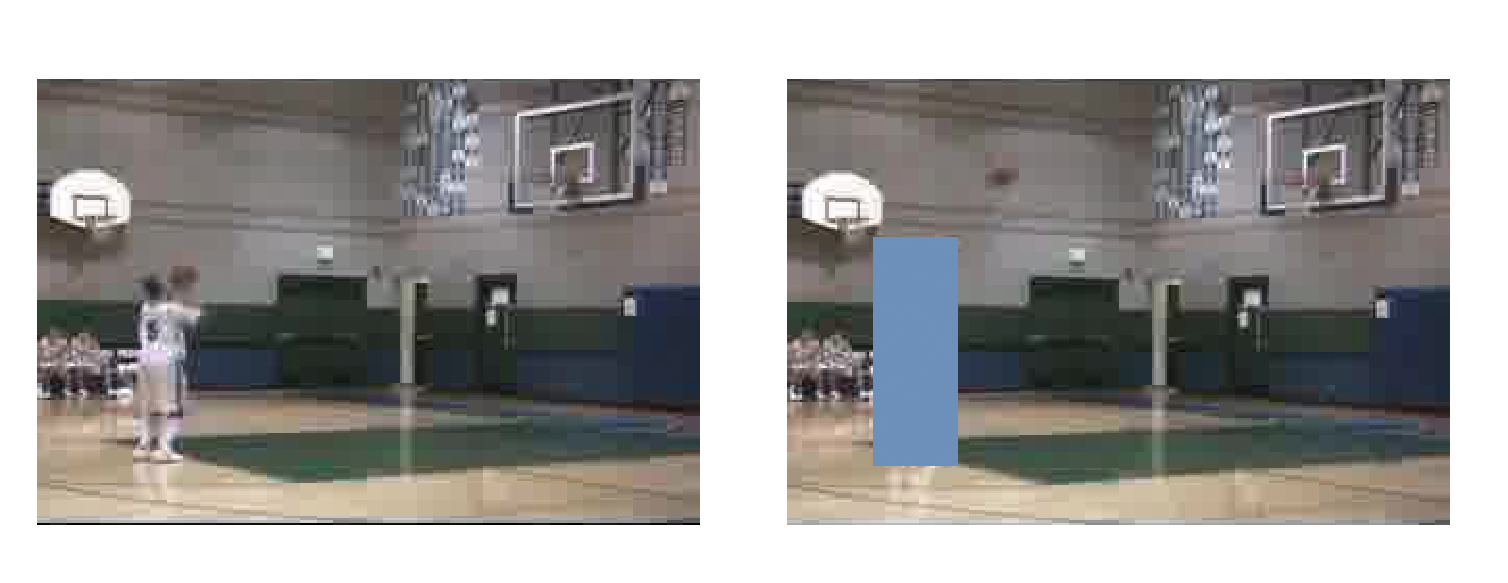
\includegraphics[scale=0.6]{imgs/bask_vs.eps}\\
(a) \hspace{2.8in} (b) \\
\caption{Background offers hints in determining human actions. (a) Sample basketball video frames. (b) Occluded video frame with player censored. The background showing the basketball court strongly suggest the action of ``playing basketball''.}
\label{bask_vs}
\end{center}
\end{figure*}
%



Based on the aforementioned intuition, the Semantic Attention ConvNet is proposed to capture the context information from both the foreground and the background. Inspired by the R*CNN~\cite{gkioxari2015contextual}, video frames are first fed into a finetuned fast RCNN framework to localize the ``foreground''\footnote{Datasets such as UCF101~\cite{soomro2012ucf101} and HMDB51~\cite{Kuehne11} do not provide bounding boxes annotation. Approximately one thousand viedo frames ares manually labeled by us to finetune the fast RCNN network. The output bounding box with the highest RCNN confidence score within a video frame is treated as the `foreground' in our framework.} with a bounding box, which is termed the {{primary region}}. Subsequently, approximately $10$ {{secondary regions}} per video frame are obtained with the Selective Search algorithm \cite{van2011segmentation} with varying intersection of Union (IoU) values with the primary region bounding box. Each testing image frame is fed into convolution layers with the RoiPooling\cite{girshick2016region} with the extracted primary region and secondary regions bounding boxes, as illustrated in Figure~\ref{basic_framework}. With the optional optical flow inputs, a combined framework can take advantage of even more spatio-temporal contexts, as shown in Figure~\ref{final_framework}. After the final stages of the RGB image stream and optical flow image stream, a fusion layer is added to account for the contributions from both streams, on which the final predictions are based.

%\noindent The major contributions of the proposed Semantic Attention ConvNet are:
The major contributions of the proposed Semantic Attention ConvNet are:
\noindent 
%
\begin{itemize}[leftmargin=*,itemsep=0cm,topsep=0cm,parsep=0cm] %enumerate
%\setlength\itemsep{0em}
%\itemsep0em
%
\item More informative spatio-temporal contexts (visual semantics and attention) are incorporated via the combination of primary region and secondary regions. 
\item The proposed flexible two-stream framework is compatible with both RGB video frame inputs and optical flow frame inputs. 
\item Even with a single RGB frame per video as input\footnote{No optical flow inputs in this particular experimental setting. The computational expensive optical flow extraction step is omitted to simulate practical applications with limited computing power.}, the proposed Semantic Attention ConvNet achieves $78.8\%$ accuracy on UCF101~\cite{soomro2012ucf101} benchmark, 
\item Empirical comparison of the Semantic Attention ConvNet based feature encoding is carried out, and the optimal one is determined, i.e., direct concatenation of VGG-16~\cite{simonyan2014very} ``fc6'' outputs.
\item An extension of the Attention ConvNet with additional iDT features ~\cite{wang2013action} is proposed, achieving even higher overall recognition accuracy.
%
\end{itemize}
%



%
The rest of this paper is organized as follows. Section~\ref{sec:related} reviews the recent research work in human action recognition, and Section~\ref{sec:attentionNet} introduces the Semantic 
Attention ConvNet. In Section~\ref{sec:experiments}, experimental results are presented based on the challenging UCF101~\cite{soomro2012ucf101} and HMBD51~\cite{Kuehne11} datasets. Finally, conclusions are drawn and the paper is summarized in Section~\ref{sec:conclusions}.
%
%------------------------------------------------------------------------
\section{Related Work}\label{sec:related}
%
Action recognition is an highly active research field in computer vision. There are mainly two types of methods: the conventional shallow feature based ones (\eg, \cite{wang2011action, wang2013action, dalal2006human}) and the deep neural network based ones. 

%
Approaches of the former type typically reply on handcrafted features\footnote{Such as, Motion Bounding Histogram (MBH)~\cite{dalal2006human}, Histogram of Oriented Gradient (HOG)~\cite{dalal2005histograms} and Histogram of Optical Flow (HOF)~\cite{chaudhry2009histograms}.} and various feature representations, such as Bag of Features (BoF)~\cite{nowak2006sampling}, Fisher Vector~\cite{perronnin2010improving} or VLAD~\cite{jegou2010aggregating}, followed by a conventional classifier such as the Support Vector Machine (SVM)~\cite{cortes1995support}. The improved Dense Trajectory (iDT)~\cite{wang2013action} method is the current state-of-the-art among this type, in which the optical flow is utilized to estimate dense trajectories, followed by HOG, HOF and MBH feature extractions around the trajectories, sub-sampling with Principal Component Analysis (PCA), encoding with a Gaussian mixture model (GMM), and finally classification with a linear SVM. Although the improved Dense Trajectory (iDT)~\cite{wang2013action} method accomplishes very high recognition accuracy, the estimation of dense trajectories and the generation of multiple features incur significant computational cost. 


%
Inspired by the success of deep learning in tasks such as classification, detection, semantic segmentation, many researchers have attempted to incorporate deep architectures for action recognition. A major difference between image based tasks and video based tasks is the extra temporal information in videos, which is often considered critical for action recognition. 

%
There are many previous research work proposing to capture the complementary information from still frames and motion between frames. \cite{karpathy2014large} extends the connectivity of a convolution neural network in time domain to take advantage of local spatio-temporal information. The late fusion method proposed in this paper is widely used in later works. Another contribution in~\cite{karpathy2014large} is that the author released a very large Sports-1M dataset, which contains 1.1 million YouTube videos belonging to 487 classes. The result in this work is humble, indicating that the motion is not captured completely. 

One of the most successful architecture in action recognition is two-stream network~\cite{simonyan2014two}. In that paper, the author use one CNN stream with the RGB frame as input to capture spatial information and another CNN stream with the stacked optical flow as input to capture temporal information. At the end of the last softmax layer, a score fusion method is established to merge spatio-temporal information. There are many methods based on it~\cite{sun2015human, WangQT15a, Feichtenhofer16, wang2016two, wang2016temporal} and achieve good results on HMDB51~\cite{Kuehne11} and UCF101~\cite{soomro2012ucf101}. Besides these approaches,  The C3D architecture proposed in~\cite{Tran_2015_ICCV} is proved to be a good tool of extracting features for video.  In this paper, the author extends traditional two dimensional convolution to three dimensional convolution, which captures spatial-temporal information adequately. Instead of using short time clips as input, in~\cite{wang2016temporal} the author proposes Temporal Segmental Network (TSN), which focus on  long-range temporal structure modeling. With the help of several good practices, this method achieves the state-of-the-art performance on the datasets of UCF101~\cite{soomro2012ucf101} and HMDB51~\cite{Kuehne11}. 

Since there are multiple cues in a still image, it's feasible to run action recognition on images. R*CNN~\cite{gkioxari2015contextual} is a outstanding work in this field, in which RCNN is adapted to multiple proposal regions and achieves good result on annotated PASAL VOC action dataset~\cite{everingham2010pascal}. Different from this method, our proposed method deploys on video action recognition task, and the two video datasets have no ground truth bounding boxes. 
The most related to our work is Two-Stream SR-CNN~\cite{wang2016two}. which incorporates human and object detection results into the two-stream framework. Our proposed work differs from Two-Stream SR-CNN in three folds: (1) We leverage several methods to 
explore cues in optical flow image, rather than using the same cues with RGB data in SR-CNN. (2) Instead of solving a dynamic programming problem to locate person, we fine-tune on Faster RCNN~\cite{ren2015faster} to obtain person position.

Another work that's similar to our method is Dynamic Network~\cite{bilen2016dynamic}, in which the author summarize the cues and information in 
video clips into a dynamic image obtained through the parameters of a ranking
machine that encodes the temporal evolution of the frames of the video, then 
feeds the dynamic image into a well-developed ConvNet to predict the label of
the video. The idea that encoding the cues of the video into a image is just
similar to the thoughts behind our method. 

%-------------------------------------------------------------------------
\section{Our Method}\label{sec:attentionNet}
In this section we elaborate our method, which is shown in Figure~\ref{basic_framework} (basic architecture) and Figure~\ref{final_framework} (full pipeline). First we introduce the basic architecture below. Given an Image $I$, we first feed it into a fine-tuned Faster RCNN~\cite{ren2015faster} and Selective Search~\cite{uijlings2013selective} pipeline to obtain primary region and candidate proposal regions, respectively. Then we input these annotations and $I$ to an adapted VGG16 network~\cite{simonyan2014very}. After the fifth convolutional layer (conv5), a ROI Polling layer is established to reuse learned feature map in primary region and secondary regions. Then primary region and secondary regions are fed into three fully connected layers separately. After obtaining maximum among secondary region scores, we add up it and primary score. Finally a softmax operation is established to transform scores into a probabilities, which can be used to classify video. Our full pipeline contains two ways of basic architecture: the one with RGB input and the one with optical flow image input. At the end of pipeline, a fusion scheme is set to predict the final prediction. Each part of implementation is detailed below.
%------------------------
\begin{figure*}[!htbp]
	\begin{center}
		\includegraphics[scale=0.25]{imgs/basic_framework.eps}
		\caption{The basic architecture of semantic attention network. }
		\label{basic_framework}
	\end{center}
\end{figure*}
%-------------------------------------------------------------------------
\subsection{Bounding Boxes Generation}\label{sec:obtain_bbox}
Since the two main benchmarks of human action recognition in video is unlabeled with bounding boxes,
we come up a solution to use Faster RCNN to annotate them. We first add bounding boxes manually for $Ann_{U}$ RGB frames in training set of UCF101~\cite{soomro2012ucf101}. When annotating, we only label the bounding box that contains the person in foreground. We then fine-tune on Faster RCNN using only two classes: background and person. When testing, we choose the box with the max score as the annotation of the frame. In this way we want to train a model that circle out actors in videos automatically. Compared with using pre-trained model directly, our method can annotate person in video more accurately.

In order to obtain secondary regions, we first run Selective Search~\cite{uijlings2013selective} in RGB frame $I$ to collect the set of region proposals. Then we choose the regions which have an overlap with primary region and the regions that have no overlap with primary region but  area large than $Area_{low}$. Formally, these regions can be defined as $Sec(r;I)$:
$$Sec(r;I)={s\in{S(I)}:overlap(s,r)\in{[l,u]} || A(s)>A_{low}},$$
where $r$ is the primary region in $I$, $S(I)$ is the selective search results of $I$,  $overlap(s; r)$ denotes the overlap ratio between region $s$ and $r$, and $A(s)$ is the area of region $s$.

When coming to optical flow image, it has no distinct secondary regions since in the flow image the still objects and background information are wiped away. We find that during a small temporal interval, the displacement of background is usually tiny. Based on this observation, we reuse bounding boxes of secondary region from contiguous RGB frame. Specifically, for the $i$th optical flow frame $o_{i}$ of a video $V$, we use secondary regions of $i+1$th RGB frame of $V$ as $o_{i}$'s secondary regions. For the primary region of optical flow image, we propose two approaches to obtain it: 1). We get the rectangle region with the largest average intension as the bounding box. 2). We reuse the primary region of the two RGB frames where the optical flow is calculated . We will compare the result of these two approaches in experiment section. Over all, by setting primary region and secondary regions reasonably for optical flow images, we extend the concept of cues and contexts to flow space. 

%-------------------------------------------------------------------------
\subsection{Learning Representations Using ConvNet}
After obtaining bounding boxes, we feed the annotated image into a convolution network (ConvNet) to learn a representation of the image. In this work we use VGG-16 architecture because of its good performance and relatively low time-cost. In order to train the secondary regions effectively, we adopt ROI pooling in our work as in~\cite{gkioxari2015contextual}. Specifically,  we replace the last pooling layer in VGG16 with the ROI pooling layer, having a convolution layer and annotated region data as input. With it, each region generates a fixed-size feature map which can be fed into fully connected layer. Since the feature maps are all cropped from the feature map at the bottom (For example, the output of the pool5 layer for VGG-16), this implementation is very efficient. 

After ROI pooling layer, we train primary region and secondary regions separately to exploit potential cues and keep the learning process of primary region clean. We feed the primary region and secondary regions to a three fully connected layers and generate scores, respectively. The only difference is that we add a max operation on secondary region stream to obtain max score. Then this max score is summed with primary region score with weights. At the end, we deploy a softmax function on score to get the probabilities of each class. We classify the instance to the class with the max probability. In addition to softmax, we explore another classifier to fusion features of two ways networks. See the discussion in Section~\ref{sec:fusion}.

%-------------------------------------------------------------------------
\subsection{Multi-task Learning}
In order to learn the class of video and the accurate position of bounding box 
synchronously, we adopt multi-task learning method to minimize the loss of the classification and loss of the bounding box regression at the same time. Given 
an image $I$, the final loss $L_{final}$ is the weighted sum of the loss of classification $L_{cls}$ and the loss of bounding box regression $L_{bbox}$:
$$L_{cls} = 1\times L_{cls}(I) + \alpha\times L_{bbox}(r;Sec(r;I)),$$
where $\alpha$ and $1$ are the weight of $L_{bbox}$ and $L_{cls}$, respectively. $Sec(r;I)$ is the secondary regions of $I$. Here we set the weight of $L_{cls}$ to 1 for the convenience of calculation. 
%-------------------------------------------------------------------------
\subsection{Feature Fusion Schemes}\label{sec:fusion}
In this subsection we introduce the feature fusion schemes for primary region stream ConvNet and secondary region stream ConvNet. we propose two approaches here: 1). For features extract from fully connected layers, we concatenate features from primary region and secondary regions, then use a  linear SVM to classify them. 2). For scores that obtained after softmax layer, we use either weighted summing or a linear SVM to see whether method works best.
%-------------------------------------------------------------------------
\subsection{Combination of RGB Data and Optical Flow Data}
In the subsections above, we discussed the basic framework of our method. Although we show our framework using RGB data, we claim here that the input of the framework can also be optical flow data. Inspired by the popular Two-Stream approach in action recognition task, we feed RGB data and optical flow data into our basic framework separately, then combine the outputs of these two networks, as shown in Figure~\ref{final_framework}. For each video, $t_{1}$ frames of RGB data and $t_{2}$ frames of optical flow data are fed into the basic architecture respectively.  Then we merge extracted spatio-temporal features using a fusion scheme posted in Section~\ref{sec:fusion} to get final prediction.
%------------------------
\begin{figure*}[!htbp]
	\begin{center}
		\includegraphics[scale=0.23]{imgs/final_framework.eps}
		\caption{The framework of combining RGB data and optical flow data.}
		\label{final_framework}
	\end{center}
\end{figure*}
%-------------------------------------------------------------------------
\section{Experiments}  \label{sec:experiments}
%
\subsection{Datasets}
We evaluate our method on UCF101~\cite{soomro2012ucf101} and HMDB51~\cite{Kuehne11} action recognition benchmarks. UCF101~\cite{soomro2012ucf101} contains 101 action classes and 13,320 video clips collected from YouTube, which mainly contains five types of action categories: 1) Human-Object Interaction; 2) Body-Motion only; 3).Human-Human Interaction; 4).Playing Musical Instruments; 5).Sports. In each of 101 class, videos are grouped into 25 groups, where each group consist of 4 to 7 videos. HMDB51~\cite{Kuehne11} contains 6766 videos clips from movies and YouTube, annotated into 51 action classes. The actions categories can be grouped in four types: 1) Facial actions; 2) General body movements; 3) Body movements with object interaction; 4) Body movements for human interaction. Both datasets have 3 splitting scheme. We first test our approach on the first split following the standard evaluation protocol. Then in order to fairly compare with the other published methods, we report our average accuracy over three splits.

%-------------------------------------------------------------------------
\subsection{ConvNet Configuration}
Our implementation is built on R*CNN, in which the VGG-16 network is used to train and test our method. Instead of using max pooling, a ROI pooling layer is established as pool5 to classify the multiple ROI regions. After that layer, we set up two ways of fully connected layer to learn primary region and secondary regions separately. We calculate the loss of classification and loss of bounding box regression and sum up them with a weight. 

Basically, we train our architecture with stochastic gradient descent (SGD) using back propagation (BP). We set initial learning rate to 0.0001 and decline it to 1/10 of it after every 30000 steps. We set the batch size to 256 and use 2 images per batch. In total, we train for 200K iterations. 

For RGB data, we randomly choose $t_{1}$ frames from each training video as input. For optical flow data, we choose $t_{2}$ frames from each video, as shown in Figure~\ref{final_framework}. When testing, we input testing image into the architecture and fusion outputs of RGB and flow network to make final prediction. 
%-------------------------------------------------------------------------

\subsection{Training and Testing Settings}
In the training procedure, $t_{1}$ RGB frames and $t_{2}$ flow frames with equal temporal spacing in each training video are selected. We choose $t_{1}={1,2,4,8}$ and fix $t_{2}$ to 10. when testing, we sample 25 frames RGB data and flow data for each testing video according to the settings in~\cite{simonyan2014two}. As shown in Figure~\ref{num_frames_accu}, increasing the number of training frames from each video doesn't increase the accuracy observably. We think the causation of this is that the video clips in these two datasets are short (average length of a video is 5 seconds), one frame is enough to capture cues and contexts in a video and extra frames only introduce noise to the data. We use one frame from each training video in the rest of the paper. 
\begin{figure}
	\begin{center}
		\includegraphics[scale=0.5]{imgs/num_frames_accu.eps}
		\caption{Results on UCF101 (split 1) using different number of RGB frames as input.}
		\label{num_frames_accu}
	\end{center}
\end{figure}
%------------------------------------------------------------------
\begin{comment}
\begin{table}
	\begin{center}
		\begin{tabular}{|l|c|}
			\hline
			\#frames  & Accuracy\\
			\hline												
			1										& 74.8\% \\
			2										& \textbf{76.8}\% \\
			4										& 75.6\% \\
			8										& 76.6\% \\
			\hline
		\end{tabular}
	\end{center}
	\caption{\textbf{Results on UCF101(split 1) using different number of RGB frames as input.} }
	\label{table:t1}
\end{table}
%--------------------------------------------------------------------
\end{comment}
\subsection{Evaluation on Human Body Detection}
In this subsection we conduct the human body detection and evaluate its effect on the final result. We label 1000 RGB images, i.e., $Ann_{U}$ is 1000, to run transfer learning on Faster RCNN. After fine-tuning the Faster RCNN network, we input a test image to the network and select the bounding box with the highest score as the primary region, which is shown with a red box in each sub figure.In each row, the first two samples are correctly annotated (with a green box outside) and the third sample is wrongly annotated (with a red box outside). 

From the Figure~\ref{good_bad_example} we find that the accuracy of annotation effects the final result heavily. For example, in $(c)$, a hand of a person playing the bowling (the true label of this frame) is detected and its pose is similar to pose in HeadMessage videos the ConvNet has seen, thus the test label is set to HeadMessage. In $(f)$, the annotator detected a small part of a green tree, which is similar to green grasses in WalkingWithDogs videos. In $(i)$, a white chopping board similar to the snowfield is detected so the ConvNet classed this frame to Skiing. These examples show that The annotator is vital for the action recognition task.
%\begin{figure*}[!htbp]
\begin{figure*}
	\begin{center}
		\includegraphics[scale=0.42]{imgs/good_bad_example.eps}
		\caption{The human detection result. Note the first two column of each row , colored in green ,are rightly labeled data,  the third column of each row, colored in red, are wrongly labeled data. At the top of each subplot, there is a test class name and its confidence. The true label of these images are (from left to right, top to bottom): Archery, CleanAnjerk, Bowling, BlowingCandles, Drumming, Basketball,  CliffDiving, Basketball, CuttingInKitchen, BlowDryHair, BoxingPunchingBag, WritingOnBoard, BabyCrawling, Billiards and Biking.}
		\label{good_bad_example}
	\end{center}
\end{figure*}
%-------------------------------------------------------------------------
%\subsection{Evaluation on the number of frames to choose}
%\begin{figure}[h]
%\begin{center}
%\includegraphics[scale=0.5]{imgs/example.eps}
%\caption{\textbf{The results using different numbers of frames.} }
%\end{center}
%\end{figure}
%-------------------------------------------------------------------------
\subsection{Evaluation on Primary Region of Optical Flow}
As discussed in Section~\ref{sec:obtain_bbox}, we use two approaches to get the primary region of optical flow image. The result is shown in Figure~\ref{table:obtain_bbox}. The approach reusing bounding box of RGB image it better, which indicates that the cues in RGB data is more useful then intension of optical flow. 
\begin{table}
	\begin{center}
		\begin{tabular}{|l|c|c|}
			\hline
			Method 	& Accuracy ($u$ channel)	& Aracy ($v$ channel)\\
			\hline												
			1)		& 75.3\% 				& 75.3\% \\		
			2)		& \textbf{76.2\%} 	& \textbf{77.4\%} \\		
			\hline
		\end{tabular}
	\end{center}
	\caption{Comparison of optical results using different primary region annotation methods. In 1), a rectangle with max average intension is selected as the primary region; in 2), the bounding box of corresponding RGB frame is selected as the primary region. we conduct experiments on $u$ channel and $v$ channel separately. See detailed description in Section~\ref{sec:obtain_bbox}}
	\label{table:obtain_bbox}
\end{table}
%-------------------------------------------------------------------------
\subsection{Evaluation on Network Parameters}
In this subsection, we will show results on split1 of UCF101~\cite{soomro2012ucf101} using only RGB data with different network parameters, including $\alpha$, the weights of two losses and dropout ratios.
\subsubsection{Weight of Bbox Regression Loss $\alpha$}
In this experiment, we set the weight of classification loss to 1 and change the weight of bbox regression loss. The result is shown in Table~\ref{table:alpha}. From the result, we find that setting the weight of classification loss and bbox regression loss to 1:0.3 achieve the best result, indicating that different losses have different contributions in back propagation. We use this ratio in the rest of this paper.
\begin{table}
	\begin{center}
		\begin{tabular}{|l|c|}
			\hline
			value of $\alpha$ & Accuracy\\
			\hline												
			0										& 74.8\% \\
			0.3										& \textbf{76.8}\% \\
			0.5										& 75.6\% \\
			0.8										& 76.6\% \\
			1.0										& 74.3\% \\
			\hline
		\end{tabular}
	\end{center}
	\caption{Comparison of results using different weight of loss of bounding box regression on RGB data of UCF101~\cite{soomro2012ucf101} split1. We fix the weight of loss of classification to 1.0 and change the weight of bbox regression loss $\alpha$. }
	\label{table:alpha}
\end{table}
\subsubsection{Dropout}
Dropout is an important technique in deep convolutional network, which can avoid overfitting correctly. In this part, we conduct on different dropout ratios when training the network. As shown in Table~\ref{table:dropout}, we achieve the best result when set dropout ratio to 0.6. Surprisingly, we only get humble 37.7\% when set dropout to 0.9 even after 200K iteration. Since 0.9 dropout ratio achieves quite good result on two-stream architecture (See Table 1 (a) in~\cite{simonyan2014two}), it indicates that multi-task architecture is more difficult to learn and is  less likely to get overfitting. 
\begin{table}
	\begin{center}
		\begin{tabular}{|c|c|}
			\hline
			Dropout ratio 							& Accuracy \\		
			\hline												
			0.5										& 75.6\% \\
			0.6										& \textbf{76.7}\% \\
			0.9										& 37.7\% \\
			\hline																				
		\end{tabular}
	\end{center}
	\caption{Comparison of results using different dropout ratios on RGB data of UCF101~\cite{soomro2012ucf101} split1. }
	\label{table:dropout}
\end{table}
%-------------------------------------------------------------------------
\subsection{Evaluation on Fusion Methods}
As discussed in Section~\ref{sec:fusion}, we use different methods to fusion the result of primary region and secondary regions. In Table~\ref{table:fusion_ps}, we find that results with softmax operation are the best. The feature of fc6 layer and fc7 layer are worse than score layer features and softmax outperforms SVM on score layer features.  
\begin{table}
	\begin{center}
		\begin{tabular}{|l|c|}
			\hline
			Fusion method							& Accuracy \\		
			\hline												
			fc6 + SVM								& 61.1\% \\
			fc7 + SVM								& 66.5\% \\
			score + SVM								& 73.7\% \\
			score + softmax 						& \textbf{75.9}\% \\
			
			\hline																				
		\end{tabular}
	\end{center}
	\caption{Comparison of different fusion method on RGB data of UCF101~\cite{soomro2012ucf101} split1. For both SVM and softmax algorithm, we extract target features from training dataset in both primary region network and secondary regions network and then concatenate them to train a classifier. Then we do the same thing on testing image to predict the class.}
	\label{table:fusion_ps}
\end{table}
%-------------------------------------------------------------------------
\subsection{Comparison with the Dynamic Image Networks}
In this subsection we compare the results of our method with the dynamic image networks. In order to compare fairly, we only use the RGB data as input to our method.
Table~\ref{table:compare_din} shows the results of our method and dynamic image networks. we find
that our method outperforms the dynamic image networks. This indicates that 
our method to encode the cues in video is effective. 
%-------------------------------------------------------------------------
\begin{table}
	\begin{center}
		\begin{tabular}{|l|c|c|}
			\hline
			Method 						& HMDB51~\cite{Kuehne11} 		& UCF101~\cite{soomro2012ucf101} 	\\
			\hline
			static RGB					& 36.7\% 		& 70.1\% 	\\
			MDI				& 35.8\% 		& 70.9\% 	\\
			MDI+static RGB & 42.8\%		& 76.9\% 	\\
			Our method                  & -				& \textbf{78.8\%} \\
			\hline
		\end{tabular}
	\end{center}
	\caption{Comparison with the dynamic image networks. Note the result of first three rows are from the origin paper of the dynamic image networks. In order to compare fairly, we only use the RGB data as input to our method.}
	\label{table:compare_din}
\end{table}

%-------------------------------------------------------------------------
\subsection{Comparison with Others' Results on Spatial Stream ConvNet}
In this subsection we compare our result on spatial stream ConvNet with other published results. Table~\ref{table:compare_spatial} shows that our method outperforms any other methods on spatial domain. This superior performance demonstrates the effectiveness of exploiting semantic attention in spatial space.
%-------------------------------------------------------------------------
\begin{table}
	\begin{center}
		\begin{tabular}{|l|c|}
			\hline
			Method 											& Accuracy	\\
			\hline
			Two-Stream~\cite{simonyan2014two}				& 73.0\% 	\\
			DIN~\cite{bilen2016dynamic}						& 76.9\% 	\\
			SR-CNN~\cite{wang2016two}						& 78.3\% 	\\
			Our method                  					& \textbf{78.8\%} \\
			\hline
		\end{tabular}
	\end{center}
	\caption{Results of spatial ConvNet on UCF101. We cite results from original papers using only spatial stream ConvNet.}
	\label{table:compare_spatial}
\end{table}
%-------------------------------------------------------------------------
\subsection{Evaluation on Fusion with Handcrafted Features}
In order to check the complement of our method with the handcrafted feature, we combine our feature with improved dense trajectory (iDT) descriptors. We first extract iDT features from UCF101~\cite{soomro2012ucf101}, then use PCA to decline the dimension to half of the origin dimension. After that, we run a Gaussian Mixture Model (GMM) with 256 components to quantize the features. Even after these operations, the dimension of iDT for each video is too large to train a classifier, so we run a PCA again to decline its dimension to 4096 or 1000. After that, we concatenate our feature with iDT features and feed them into a SVM classifier. The result is shown in Table~\ref{table:iDT}. Note that Because of dimensionality reduction, iDT only achieves 78.1\% while the accuracy reported on original paper is 85.7\%.

From the result, we can see that combining with the iDT can improve accuracy by 7.6\% at most. This indicates that our method is complementary to the handcrafted feature. 
\begin{table}
	\begin{center}
		\begin{tabular}{|l|c|c|}
			\hline
			Method 								& iDT (1000 dim) 			& iDT (4096 dim) 		\\
			\hline
			iDT 								& 77.8\% 				& 78.1\% 			\\
			iDT + fc6 							& 82.7\% 				& \textbf{85.7\%} 	\\
			iDT + fc7							& 82.9 					& 84.9\% 			\\
			iDT + score							& \textbf{84.8\%} 	& 83.9\% 			\\
			\hline																				
		\end{tabular}
	\end{center}
	\caption{Comparison of results using different ConvNet layers to fusion with iDT. In order to train faster, we decline the dimension of iDT feature to 1000 dim and 4096 dim using PCA. After that, we concatenate our feature with iDT and feed them into a SVM classifier.}
	\label{table:iDT}
\end{table}

%-------------------------------------------------------------------------
\subsection{Comparison with Published Results}
In this section we compare our method with other state-of-the-art approaches. We simply use the result from the origin papers. From the Table~\ref{table:all_result}, we find that our method is comparable with iDT and C3D, weaker than the state-of-the-art method TSN, in which the authors used a deeper network (Inception-BN) which offers a higher baseline.  Besides, the author used the spatial and temporal modality pre-training to boost accuracy, which is time-consuming.  
\begin{table}
	\begin{center}
		\begin{tabular}{|l|c|c|}
			\hline
			Method & HMDB51~\cite{Kuehne11} & UCF101~\cite{soomro2012ucf101} \\
			\hline
			iDT~\cite{wang2013action} 											& 57.2\% 	& 85.9\% \\
			Slow Fusion~\cite{karpathy2014large}   								& - 		& 65.4\% \\
			Two Stream~\cite{simonyan2014two} 									& 59.4\% 	& 88.0\% \\
			C3D (3 nets)~\cite{Tran_2015_ICCV}									& - 		& 85.2\% \\
			TSN~\cite{wang2016temporal}											& 69.4\%	& 94.2\% \\
			our results															& - 		& 85.7\% \\
			\hline
		\end{tabular}
	\end{center}
	\caption{Comparison of our method with other state-of-the-art methods. We simply use the result from the origin papers.}
	\label{table:all_result}
\end{table}

%------------------------------------------------------------------------
\section{Conclusions}\label{sec:conclusions}
In this paper we propose a semantic attentive deep learning model for action recognition in video. We first add bounding boxes to video frames, then feed annotated images into a very deep convolution network to minimize the loss using a multi-task learning method. The learned features are then combined to form the final prediction. With only RGB image as input, we can achieve 78.8\% on UCF101~\cite{soomro2012ucf101} benchmark. This result outperforms other methods based on image, indicating that our method can grasp information in video frames richly. With input of RGB image and optical flow image, our method can achieve 79.0\% on the benchmark. When combined with iDT, our method can achieve 85.7\% on the benchmark. Since our method can be input into a end-to-end architecture, in the future we will explore to find a pipeline to run our method online. On the other hand, we will investigate multi-modal method to present contexts more accurately. 
\clearpage
{\small
	\bibliographystyle{ieee}
	\bibliography{SemanticAttention_bib}
}

\end{document}

